%%%%%%%%%%%%%%%%%%%%%%%%%%%%% Define Article %%%%%%%%%%%%%%%%%%%%%%%%%%%%%%%%%%
\documentclass[12pt]{report}
%%%%%%%%%%%%%%%%%%%%%%%%%%%%%%%%%%%%%%%%%%%%%%%%%%%%%%%%%%%%%%%%%%%%%%%%%%%%%%%

%%%%%%%%%%%%%%%%%%%%%%%%%%%%% Using Packages %%%%%%%%%%%%%%%%%%%%%%%%%%%%%%%%%%
\usepackage{geometry}
\usepackage{graphicx}
\usepackage{amssymb}
\usepackage{amsmath}
\usepackage{amsthm}
\usepackage{empheq}
\usepackage{mdframed}
\usepackage{booktabs}
\usepackage{color}
\usepackage{psfrag}
\usepackage{pgfplots}
\usepackage{bm}
\usepackage{listings}
\usepackage{xcolor}
\usepackage{hyperref}
%%%%%%%%%%%%%%%%%%%%%%%%%%%%%%%%%%%%%%%%%%%%%%%%%%%%%%%%%%%%%%%%%%%%%%%%%%%%%%%

% Other Settings

%%%%%%%%%%%%%%%%%%%%%%%%%% Page Setting %%%%%%%%%%%%%%%%%%%%%%%%%%%%%%%%%%%%%%%
\geometry{a4paper}

%%%%%%%%%%%%%%%%%%%%%%%%%% Define some useful colors %%%%%%%%%%%%%%%%%%%%%%%%%%
\definecolor{ocre}{RGB}{243,102,25}
\definecolor{mygray}{RGB}{243,243,244}
\definecolor{deepGreen}{RGB}{26,111,0}
\definecolor{shallowGreen}{RGB}{235,255,255}
\definecolor{deepBlue}{RGB}{61,124,222}
\definecolor{shallowBlue}{RGB}{235,249,255}
%%%%%%%%%%%%%%%%%%%%%%%%%%%%%%%%%%%%%%%%%%%%%%%%%%%%%%%%%%%%%%%%%%%%%%%%%%%%%%%

%%%%%%%%%%%%%%%%%%%%%%%%%% Define an orangebox command %%%%%%%%%%%%%%%%%%%%%%%%
\newcommand\orangebox[1]{\fcolorbox{ocre}{mygray}{\hspace{1em}#1\hspace{1em}}}
%%%%%%%%%%%%%%%%%%%%%%%%%%%%%%%%%%%%%%%%%%%%%%%%%%%%%%%%%%%%%%%%%%%%%%%%%%%%%%%

%%%%%%%%%%%%%%%%%%%%%%%%%%%% English Environments %%%%%%%%%%%%%%%%%%%%%%%%%%%%%
\newtheoremstyle{mytheoremstyle}{3pt}{3pt}{\normalfont}{0cm}{\rmfamily\bfseries}{}{1em}{{\color{black}\thmname{#1}~\thmnumber{#2}}\thmnote{\,--\,#3}}
\newtheoremstyle{myproblemstyle}{3pt}{3pt}{\normalfont}{0cm}{\rmfamily\bfseries}{}{1em}{{\color{black}\thmname{#1}~\thmnumber{#2}}\thmnote{\,--\,#3}}
\theoremstyle{mytheoremstyle}
\newmdtheoremenv[linewidth=1pt,backgroundcolor=shallowGreen,linecolor=deepGreen,leftmargin=0pt,innerleftmargin=20pt,innerrightmargin=20pt,]{theorem}{Theorem}[section]
\theoremstyle{mytheoremstyle}
\newmdtheoremenv[linewidth=1pt,backgroundcolor=shallowBlue,linecolor=deepBlue,leftmargin=0pt,innerleftmargin=20pt,innerrightmargin=20pt,]{definition}{Definition}[section]
\theoremstyle{myproblemstyle}
\newmdtheoremenv[linecolor=black,leftmargin=0pt,innerleftmargin=10pt,innerrightmargin=10pt,]{problem}{Problem}[section]
%%%%%%%%%%%%%%%%%%%%%%%%%%%%%%%%%%%%%%%%%%%%%%%%%%%%%%%%%%%%%%%%%%%%%%%%%%%%%%%

%%%%%%%%%%%%%%%%%%%%%%%%%%%%%%% Plotting Settings %%%%%%%%%%%%%%%%%%%%%%%%%%%%%
\usepgfplotslibrary{colorbrewer}
\pgfplotsset{width=8cm,compat=1.9}
%%%%%%%%%%%%%%%%%%%%%%%%%%%%%%%%%%%%%%%%%%%%%%%%%%%%%%%%%%%%%%%%%%%%%%%%%%%%%%%

\definecolor{codegreen}{rgb}{0,0.6,0}
\definecolor{codegray}{rgb}{0.5,0.5,0.5}
\definecolor{codepurple}{rgb}{0.58,0,0.82}
\definecolor{backcolour}{rgb}{0.95,0.95,0.92}
 
\lstdefinestyle{mystyle}{
    backgroundcolor=\color{backcolour},   
    commentstyle=\color{codegreen},
    keywordstyle=\color{magenta},
    numberstyle=\tiny\color{codegray},
    stringstyle=\color{codepurple},
    basicstyle=\ttfamily\footnotesize,
    breakatwhitespace=false,         
    breaklines=true,                 
    captionpos=b,                    
    keepspaces=true,                 
    numbers=left,                    
    numbersep=5pt,                  
    showspaces=false,                
    showstringspaces=false,
    showtabs=false,                  
    tabsize=2
}
\lstset{style=mystyle}


%%%%%%%%%%%%%%%%%%%%%%%%%%%%%%%%%%%%%%%%%%%%%%%%%%%%%%%%%%%%%%%%%%%%%%%%%%%%%%%

\begin{document}
\begin{titlepage}
	\topskip0pt
	\vspace*{\fill}

	\begin{center}


		
\includegraphics[width=0.6\textwidth]{images/logo.png}

		\vspace{2cm}

		\Huge
		\textbf{Evolutionary Algorithms}
		\vspace{0.5cm}

		\Large

		\textbf{ \href{mailto:mq06861@st.habib.edu.pk}{Muhammad Meesum Ali Qazalbash - mq06861}}\\
		\textbf{ \href{mailto:@st.habib.edu.pk}{{Syed Ibrahim Ali Haider - sh06565}}}

		\today
		\vspace{0.5cm}

		CS451 - Computational Intelligence

		\vspace{0.5cm}
		\large
		Assignment 1
	\end{center}

	\vspace*{\fill}
\end{titlepage}


\setcounter{page}{2}
\tableofcontents

\chapter{Abstract}
The purpose of this assignment is to gather an insight of stochastic optimization using Evolutionary Algorithms (EA). This exercise will enable us to address some known computing problems that map to several real-world problems and are known to be computationally hard.

\chapter{Problems}

\section{Genetic Algorithm}
The genetic algorithm is a search heuristic that replicates the process of natural evolution. This is represent the class with the following attributes,
\lstinputlisting[language=python, caption= {Evolution class},linerange={16-23},firstnumber=16]{../Code/Evolution/evolution.py}
The fittest chromosome is selected the chromosome maximized by the fittness function.
\lstinputlisting[language=python, caption= {Fittest chromosome},linerange={50-56},firstnumber=50]{../Code/Evolution/evolution.py}

\newpage

The best fitness is the fitness of the best chromosome.
\lstinputlisting[language=python, caption= {Best fitness},linerange={58-68},firstnumber=58]{../Code/Evolution/evolution.py}
We randomly selects two parents and mate them to breed children. This process is repeated \lstinline|number_of_offspring| times.
\lstinputlisting[language=python, caption= {Select two parents and add their offspring to the population},linerange={140-153},firstnumber=140]{../Code/Evolution/evolution.py}

\newpage

First we select parents from population using \lstinline|selection_method1| and then the parents breed and a new chromosome enters the population which are then selected using \lstinline|selection_method2| as survivors.
\lstinputlisting[language=python, caption= {Next generation},linerange={155-172},firstnumber=155]{../Code/Evolution/evolution.py}

\newpage

The \lstinline{step} is returns the next generation and the best fitness. \lstinline{run} runs the evolution process and return the fitness of all chromosomes.
\lstinputlisting[language=python, caption= {Run the evolution},linerange={174-199},firstnumber=174]{../Code/Evolution/evolution.py}

\newpage

\subsection{Selection Schemes}
The selection scheme class caters all the selection methods. It requires two attributes first the population size and the other is fitness function.
\lstinputlisting[language=python, caption= {Selection Scheme class},linerange={6-20},firstnumber=6]{../Code/Evolution/selection_schemes.py}

\newpage

This function would select the chromosome according to their fitness values.
\lstinputlisting[language=python, caption= {Fitness proportion selection method},linerange={48-65},firstnumber=48]{../Code/Evolution/selection_schemes.py}

\newpage

The tournament selection method relies on for every chromosome it selects two random chromosome and compete them according to the fitness function and the winner gets appended to the new population.
\lstinputlisting[language=python, caption= {Tournament selection method},linerange={67-86},firstnumber=67]{../Code/Evolution/selection_schemes.py}

\newpage

Rank based selection method priorotizes the chromosome with high fitness value over low fitness one, and then randomly selects them.
\lstinputlisting[language=python, caption= {Rank based selection method},linerange={88-109},firstnumber=88]{../Code/Evolution/selection_schemes.py}
Random selection methods is just randomly selecting desired number of chromosomes.
\lstinputlisting[language=python, caption= {Random selection method},linerange={111-120},firstnumber=111]{../Code/Evolution/selection_schemes.py}

\newpage

\section{Travelling Salesman Problem}
A chromosome is represented by a list of different cities.
\lstinputlisting[language=python, caption= {Chromosome representation},linerange={18-25},firstnumber=18]{../Code/Travelling_Salesman/tsp.py}
The fitness function is the inverse of the sum of the distances between the cities in order.
\lstinputlisting[language=python, caption= {Fitness function},linerange={27-39},firstnumber=27]{../Code/Travelling_Salesman/tsp.py}

\newpage

The mutation is happening by swapping the cities in the route.
\lstinputlisting[language=python, caption= {Mutation},linerange={41-55},firstnumber=41]{../Code/Travelling_Salesman/tsp.py}
The crossover is done by randomly selecting two cities and then placing all the cities that are intermediate to reach them and placing them in the start of the tour. Rest of the cities comes in the end of the route.
\lstinputlisting[language=python, caption= {Crossover},linerange={57-76},firstnumber=57]{../Code/Travelling_Salesman/tsp.py}

\newpage

\section{Graph Coloring Problem}
A chromosome is represented using the matrix representation for graphs.
\lstinputlisting[language=python, caption= {Chromosome representation},linerange={23-33},firstnumber=23]{../Code/Graph_Coloring/graph_coloring.py}
Fitness function is defined as inverse of the number of unique individuals we have if they are valid other wise it is zero.
\lstinputlisting[language=python, caption= {Fitness function},linerange={35-51},firstnumber=35]{../Code/Graph_Coloring/graph_coloring.py}

\newpage

Crossover is done by selecting a random index and placing all the elements after that index the start of the list.
\lstinputlisting[language=python, caption= {Crossover},linerange={53-66},firstnumber=53]{../Code/Graph_Coloring/graph_coloring.py}
Mutation is done by assigning a random color to a random chromosome.
\lstinputlisting[language=python, caption= {Mutation},linerange={68-80},firstnumber=68]{../Code/Graph_Coloring/graph_coloring.py}

\newpage

\section{Knapsack Problem}
Chromosome are just a list of ones and zeros, that refers the selection of that wieght.
\lstinputlisting[language=python, caption= {Chromosome representation},linerange={17-24},firstnumber=17]{../Code/Knapsack/knapsack.py}
Fitness function return zero if the total wieght is greater than the threshold otherwise it returns the wieght.
\lstinputlisting[language=python, caption= {Fitness function},linerange={26-47},firstnumber=26]{../Code/Knapsack/knapsack.py}

\newpage

Mutation is done by randomly switching the state of the wieght.
\lstinputlisting[language=python, caption= {Mutation},linerange={49-61},firstnumber=49]{../Code/Knapsack/knapsack.py}
Crossover is done by selecting a random index and placing all the elements after that index the start of the list.
\lstinputlisting[language=python, caption= {Crossover},linerange={63-79},firstnumber=63]{../Code/Knapsack/knapsack.py}

\newpage

\section{Optimization Class}
Optimization class handles the testing of the algorithms. It requires attributes mentioned below along with their default arguments.
\lstinputlisting[language=python, caption= {Parameters},linerange={9-37},firstnumber=9]{../Code/optimization.py}

\newpage

This function would evolve the generation according to the values provided.
\lstinputlisting[language=python, caption= {Evolution},linerange={39-51},firstnumber=39]{../Code/optimization.py}
The title for the plot is generated by the following function.
\lstinputlisting[language=python, caption= {Getter for title},linerange={53-70},firstnumber=53]{../Code/optimization.py}

\newpage

The name of the file is generated by the following function.
\lstinputlisting[language=python, caption= {Getter for filename},linerange={72-87},firstnumber=72]{../Code/optimization.py}
The best so far is ploted with the following function.
\lstinputlisting[language=python, caption= {Plotter for best so far},linerange={89-111},firstnumber=89]{../Code/optimization.py}

\newpage

The average so far is ploted with the following function.
\lstinputlisting[language=python, caption= {Plotter for average so far},linerange={113-146},firstnumber=113]{../Code/optimization.py}

\newpage

\chapter{Analysis}
We tried 10 different combinations of the 5 selection schemes that are,
\begin{enumerate}
	\item Fitness Proportional Selection
	\item Rank based Selection
	\item Binary Tournament
	\item Truncation
	\item Random
\end{enumerate}

and those combinations are,
\begin{enumerate}
	\item FPS and Random
	\item Binary Tournament and Truncation
	\item Truncation and Truncation
	\item Random and Random
	\item FPS and Truncation
	\item RBS and Binary Tournament
	\item Random and Truncation
	\item Binary Tournament and FPS
	\item Binary Tournament and RBS
	\item Truncation and FPS
\end{enumerate}


\section{Graph Coloring Problem}

\subsection{Average So Far}
Again we found 2 best selection scheme combinations, which were Tournament \& Truncation, and Truncation and Truncation, with their fitness being 40. The worst selection scheme combination was Random \& Random with the fitness being 100, we also saw that FPS \& Random did not give us good results too.

\begin{figure}[!]

	\begin{minipage}{0.4\textwidth}
		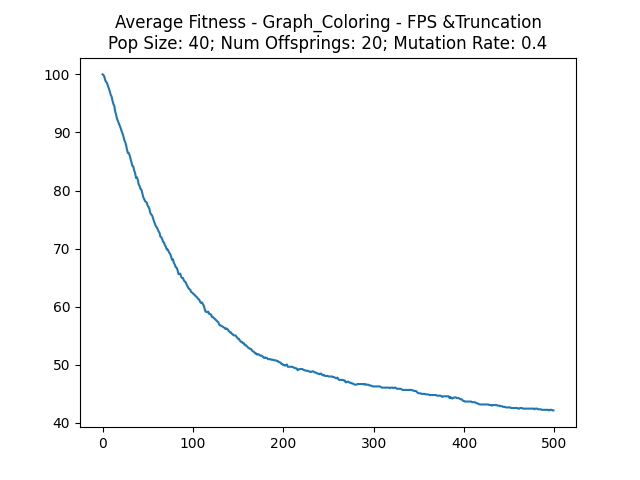
\includegraphics[width=\linewidth]{../Analysis/ASF_Graph_Coloring_0_3_40_20.png}
	\end{minipage}
	\hspace{\fill}
	\begin{minipage}{0.4\textwidth}
		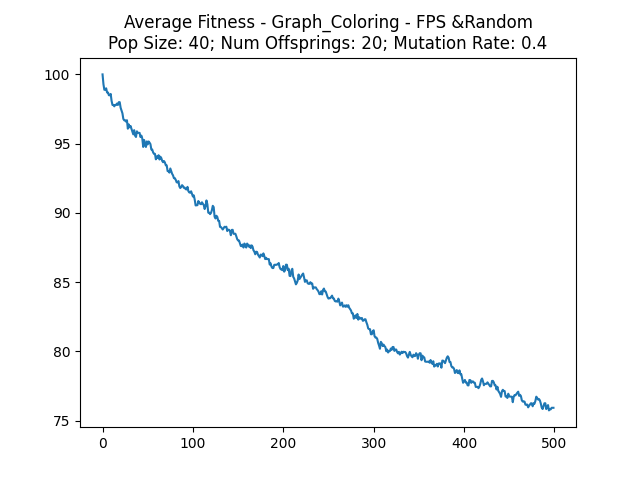
\includegraphics[width=\linewidth]{../Analysis/ASF_Graph_Coloring_0_4_40_20.png}
	\end{minipage}
	\vspace*{1cm}
	\begin{minipage}{0.4\textwidth}
		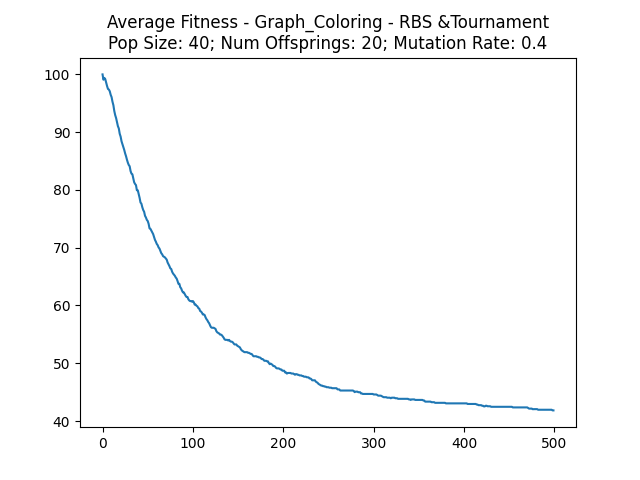
\includegraphics[width=\linewidth]{../Analysis/ASF_Graph_Coloring_1_2_40_20.png}
	\end{minipage}
	\hspace{\fill}
	\begin{minipage}{0.4\textwidth}
		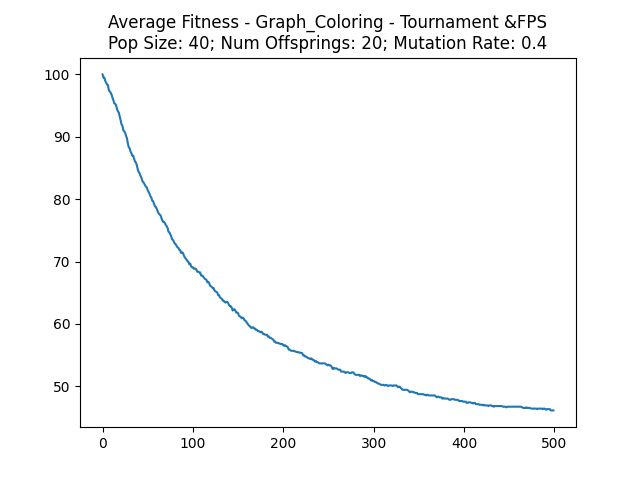
\includegraphics[width=\linewidth]{../Analysis/ASF_Graph_Coloring_2_0_40_20.png}
	\end{minipage}
	\vspace*{1cm}
	\begin{minipage}{0.4\textwidth}
		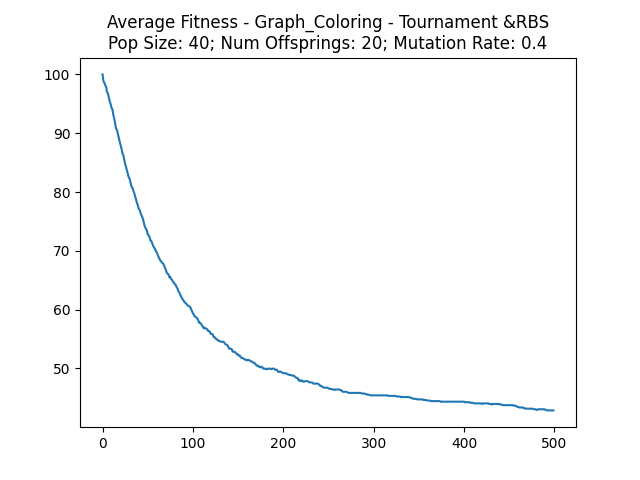
\includegraphics[width=\linewidth]{../Analysis/ASF_Graph_Coloring_2_1_40_20.png}
	\end{minipage}
	\hspace{\fill}
	\begin{minipage}{0.4\textwidth}
		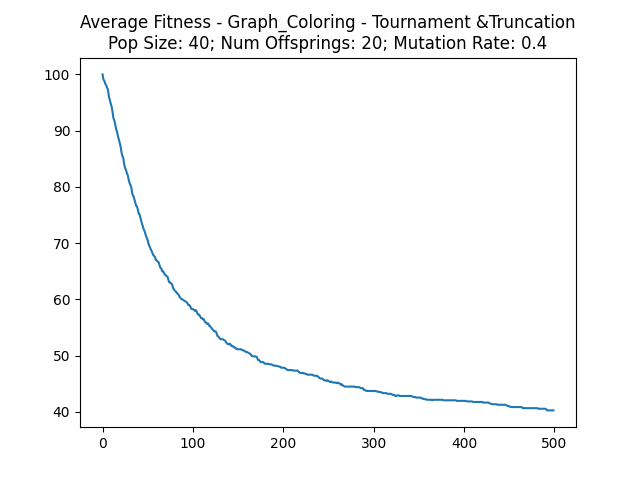
\includegraphics[width=\linewidth]{../Analysis/ASF_Graph_Coloring_2_3_40_20.png}
	\end{minipage}
	\vspace*{1cm}
	\begin{minipage}{0.4\textwidth}
		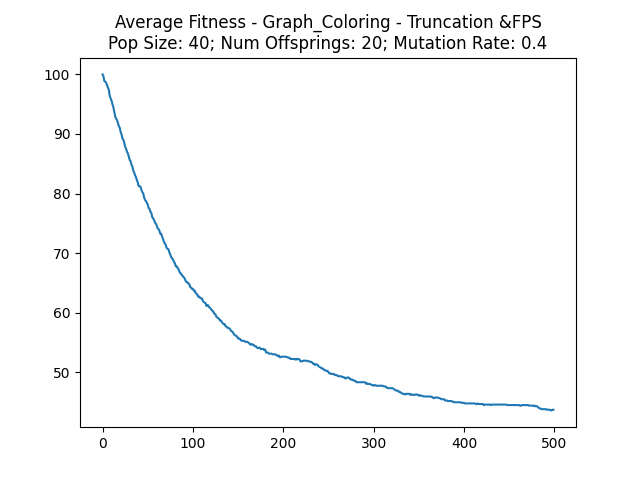
\includegraphics[width=\linewidth]{../Analysis/ASF_Graph_Coloring_3_0_40_20.png}
	\end{minipage}
	\hspace{\fill}
	\begin{minipage}{0.4\textwidth}
		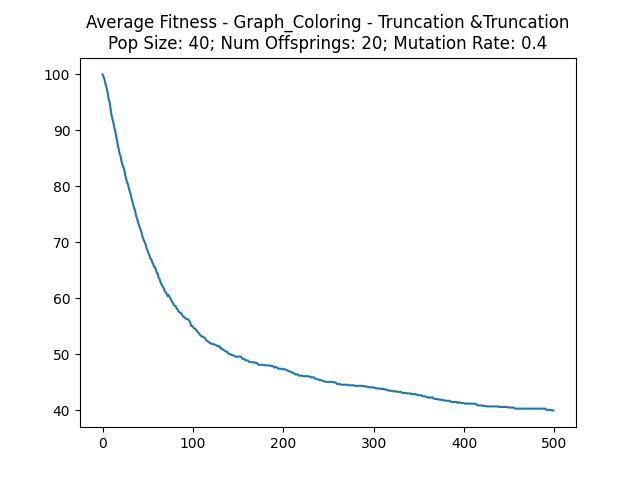
\includegraphics[width=\linewidth]{../Analysis/ASF_Graph_Coloring_3_3_40_20.png}
	\end{minipage}
	\vspace*{1cm}
	\begin{minipage}{0.4\textwidth}
		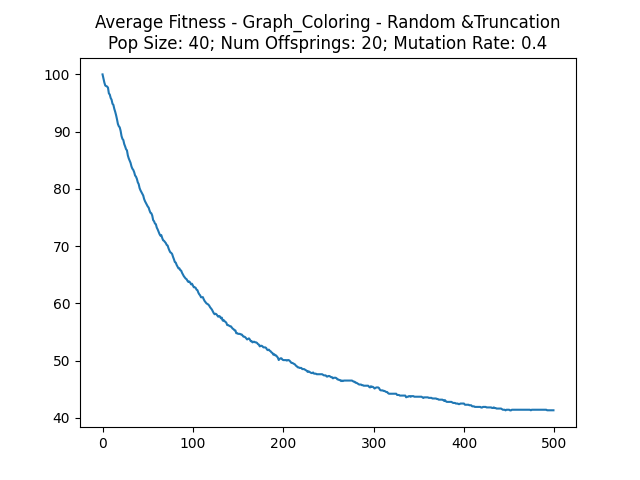
\includegraphics[width=\linewidth]{../Analysis/ASF_Graph_Coloring_4_3_40_20.png}
	\end{minipage}
	\hspace{\fill}
	\begin{minipage}{0.4\textwidth}
		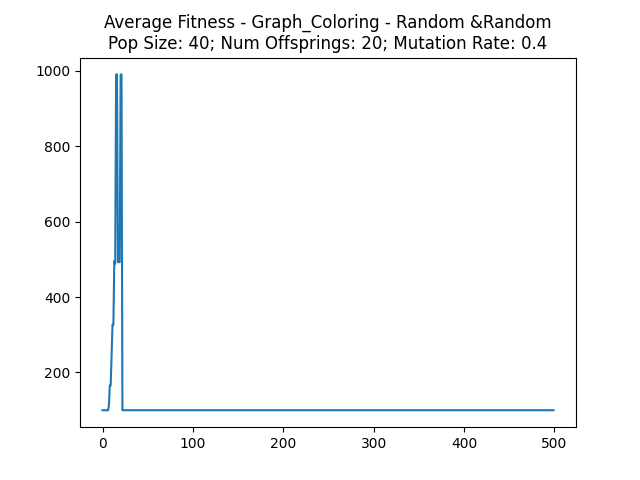
\includegraphics[width=\linewidth]{../Analysis/ASF_Graph_Coloring_4_4_40_20.png}
	\end{minipage}
	\vspace*{1cm}
\end{figure}
\newpage

\subsection{Best So Far}
We found 2 of the schemes to be best among our selection scheme combinations, Random \& Truncation and RBS \& Tournament, both of these combinations gave us a fitness level of around 34. Whereas the worst selection scheme combination was Random and Random in which the fitness that we received was 100.

The overall majority of the fitnesses were in near 36-35, these proved to be quite impressive as compared to our initial fitness values.
\begin{figure}[!]

	\begin{minipage}{0.4\textwidth}
		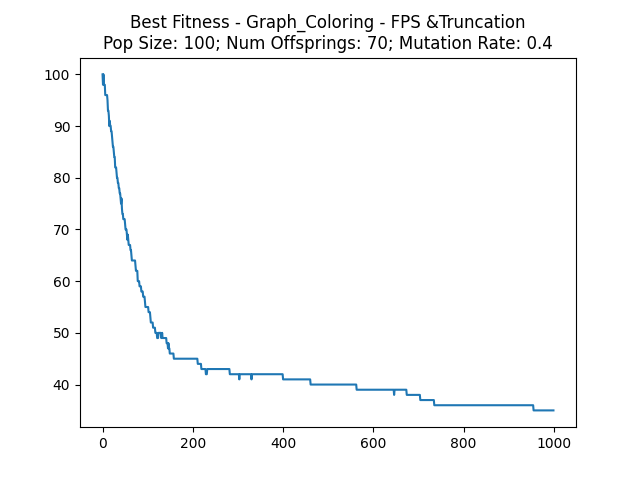
\includegraphics[width=\linewidth]{../Analysis/BSF_Graph_Coloring_0_3_100_70.png}
	\end{minipage}
	\hspace{\fill}
	\begin{minipage}{0.4\textwidth}
		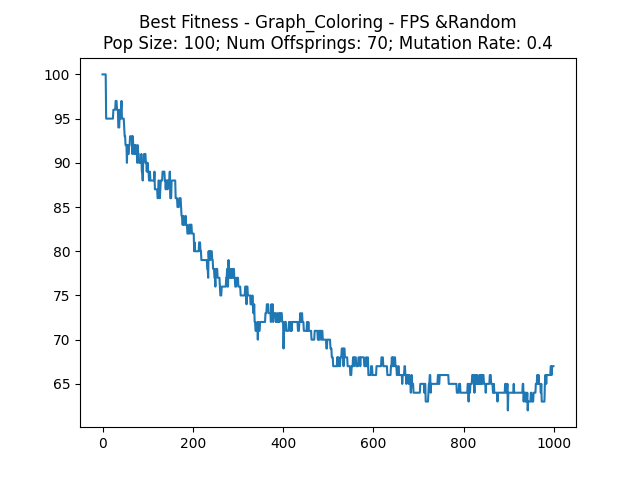
\includegraphics[width=\linewidth]{../Analysis/BSF_Graph_Coloring_0_4_100_70.png}
	\end{minipage}
	\vspace*{1cm}
	\begin{minipage}{0.4\textwidth}
		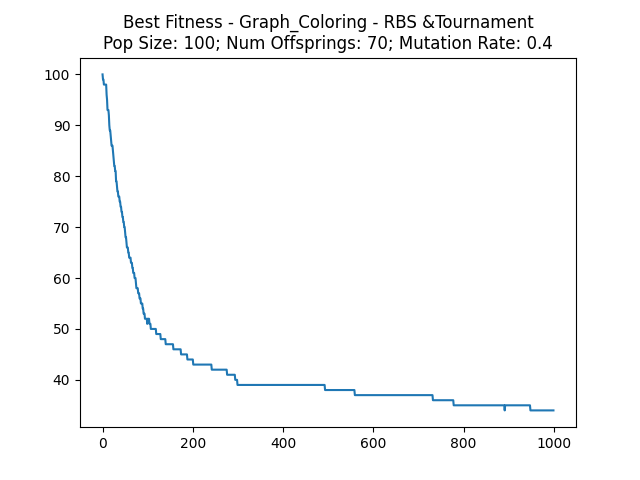
\includegraphics[width=\linewidth]{../Analysis/BSF_Graph_Coloring_1_2_100_70.png}
	\end{minipage}
	\hspace{\fill}
	\begin{minipage}{0.4\textwidth}
		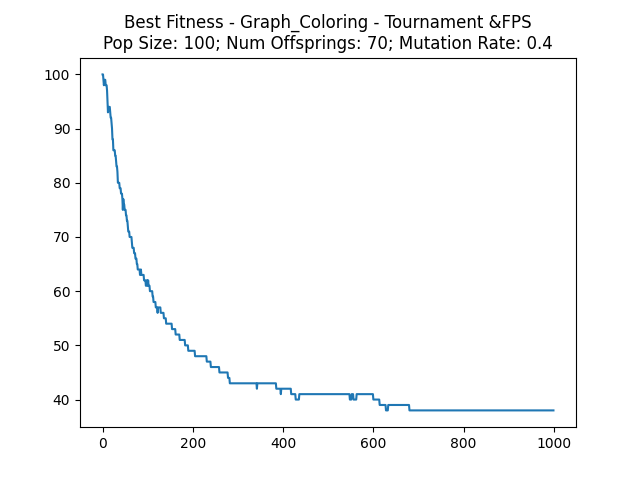
\includegraphics[width=\linewidth]{../Analysis/BSF_Graph_Coloring_2_0_100_70.png}
	\end{minipage}
	\vspace*{1cm}
	\begin{minipage}{0.4\textwidth}
		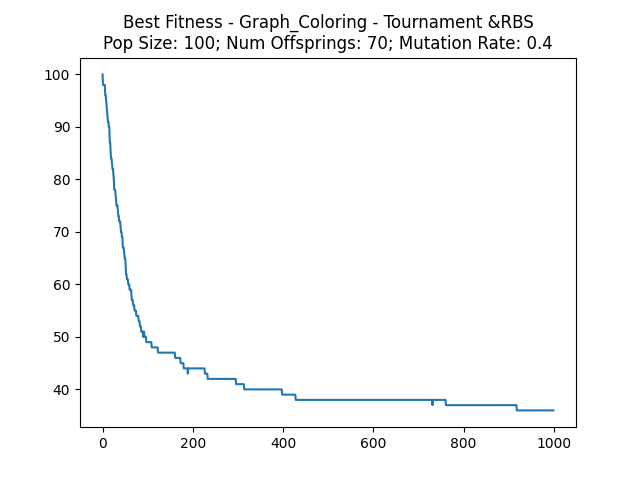
\includegraphics[width=\linewidth]{../Analysis/BSF_Graph_Coloring_2_1_100_70.png}
	\end{minipage}
	\hspace{\fill}
	\begin{minipage}{0.4\textwidth}
		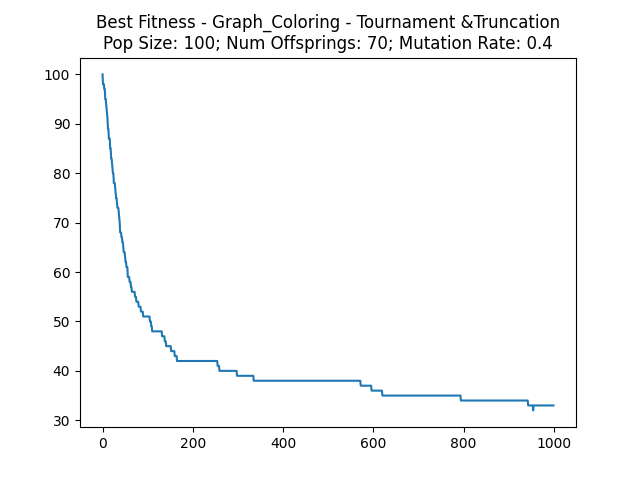
\includegraphics[width=\linewidth]{../Analysis/BSF_Graph_Coloring_2_3_100_70.png}
	\end{minipage}
	\vspace*{1cm}
	\begin{minipage}{0.4\textwidth}
		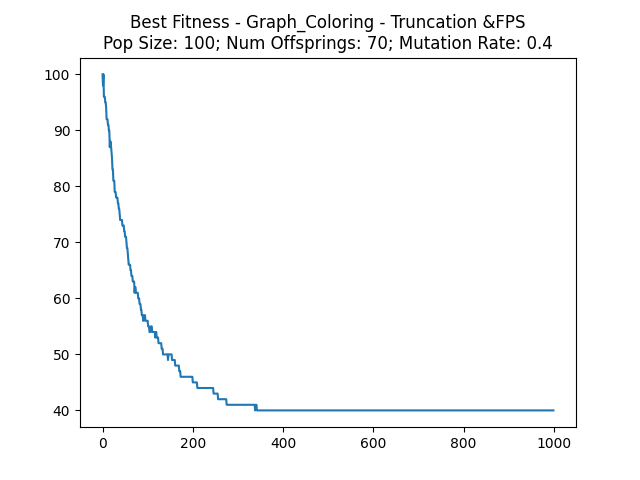
\includegraphics[width=\linewidth]{../Analysis/BSF_Graph_Coloring_3_0_100_70.png}
	\end{minipage}
	\hspace{\fill}
	\begin{minipage}{0.4\textwidth}
		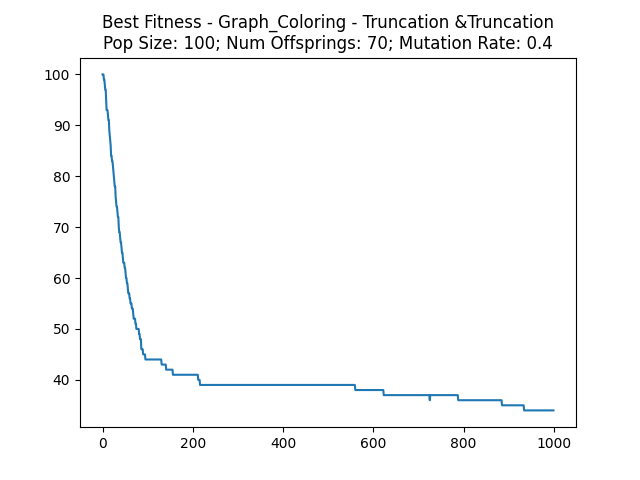
\includegraphics[width=\linewidth]{../Analysis/BSF_Graph_Coloring_3_3_100_70.png}
	\end{minipage}
	\vspace*{1cm}
	\begin{minipage}{0.4\textwidth}
		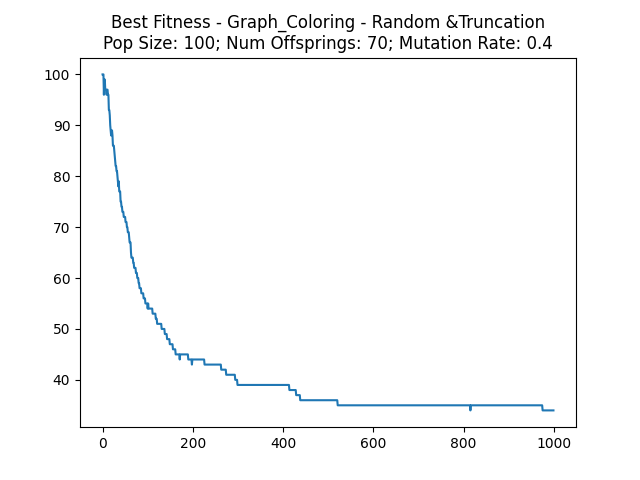
\includegraphics[width=\linewidth]{../Analysis/BSF_Graph_Coloring_4_3_100_70.png}
	\end{minipage}
	\hspace{\fill}
	\begin{minipage}{0.4\textwidth}
		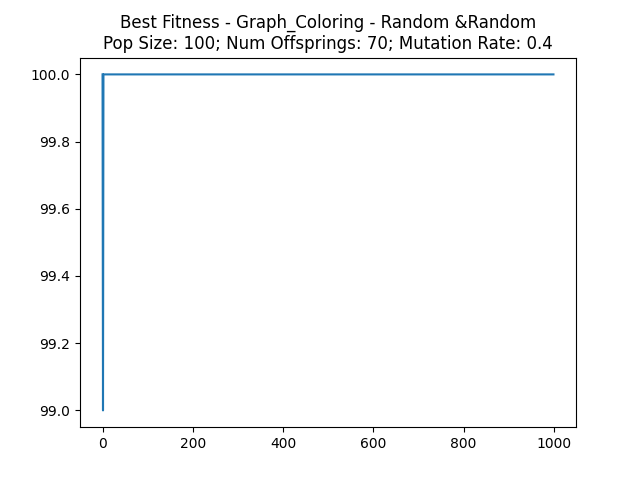
\includegraphics[width=\linewidth]{../Analysis/BSF_Graph_Coloring_4_4_100_70.png}
	\end{minipage}
\end{figure}
\newpage

\section{Travelling Salesman Problem}


\subsection{Average So Far}
The best results were given by FPS \& Truncation, and RBS \& Tournament, with both of the selected combinations having a greater depth in their trend. The worst results were given by FPS \& Random, and Random \& Random, which had chaotic results with almost no convergence

If we look at the plots of ASF on various selection schemes we again see that most of the combinations have achieved impressive fitness results, and are similar to each other as compared to their initial fitness scores.
\begin{figure}[!]

	\begin{minipage}{0.4\textwidth}
		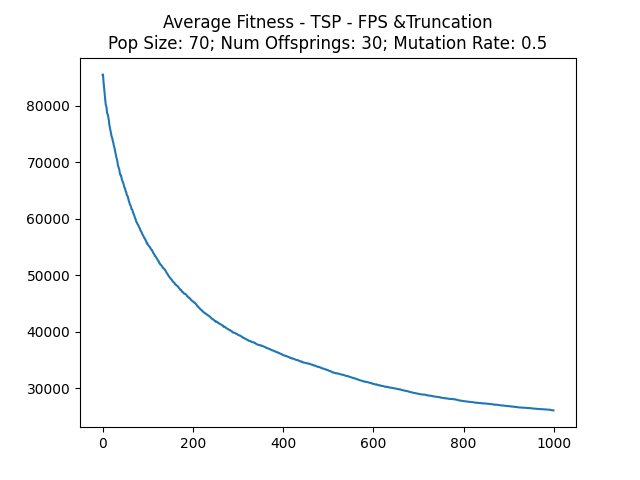
\includegraphics[width=\linewidth]{../Analysis/ASF_TSP_0_3_70_30.png}
	\end{minipage}
	\hspace{\fill}
	\begin{minipage}{0.4\textwidth}
		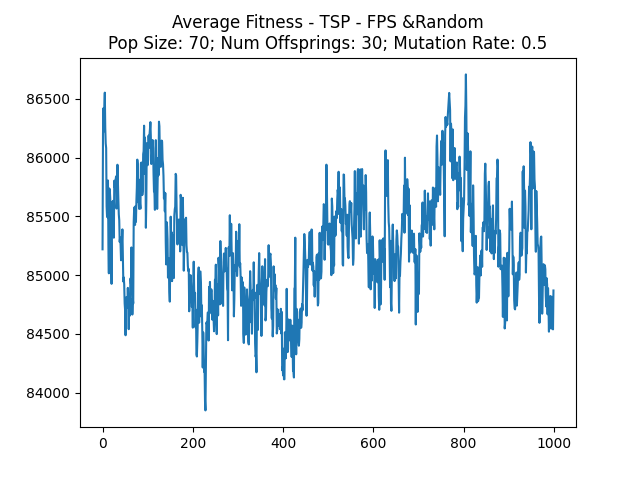
\includegraphics[width=\linewidth]{../Analysis/ASF_TSP_0_4_70_30.png}
	\end{minipage}
	\vspace*{1cm}
	\begin{minipage}{0.4\textwidth}
		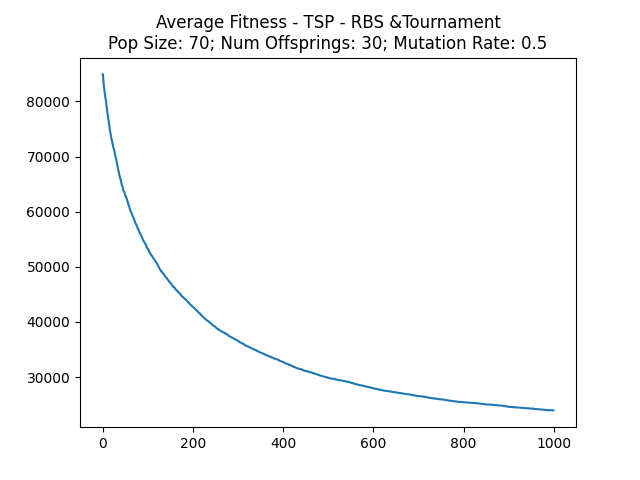
\includegraphics[width=\linewidth]{../Analysis/ASF_TSP_1_2_70_30.png}
	\end{minipage}
	\hspace{\fill}
	\begin{minipage}{0.4\textwidth}
		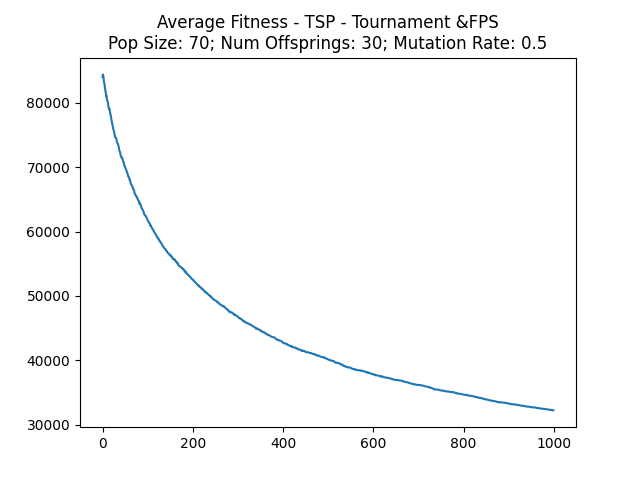
\includegraphics[width=\linewidth]{../Analysis/ASF_TSP_2_0_70_30.png}
	\end{minipage}
	\vspace*{1cm}
	\begin{minipage}{0.4\textwidth}
		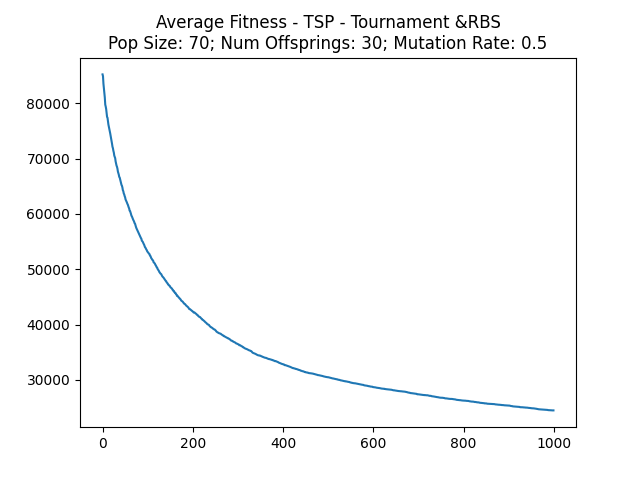
\includegraphics[width=\linewidth]{../Analysis/ASF_TSP_2_1_70_30.png}
	\end{minipage}
	\hspace{\fill}
	\begin{minipage}{0.4\textwidth}
		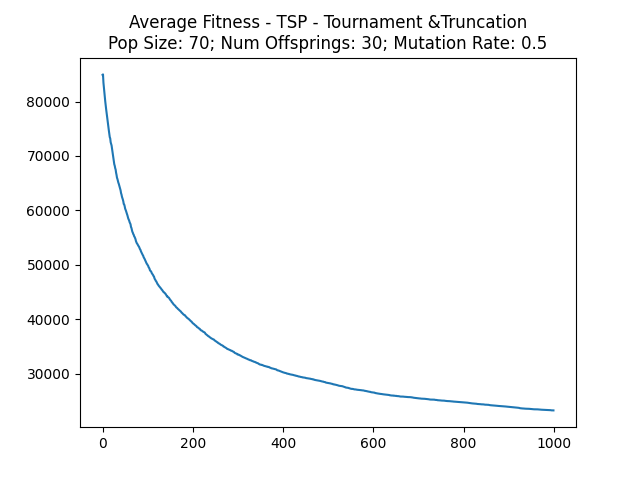
\includegraphics[width=\linewidth]{../Analysis/ASF_TSP_2_3_70_30.png}
	\end{minipage}
	\vspace*{1cm}
	\begin{minipage}{0.4\textwidth}
		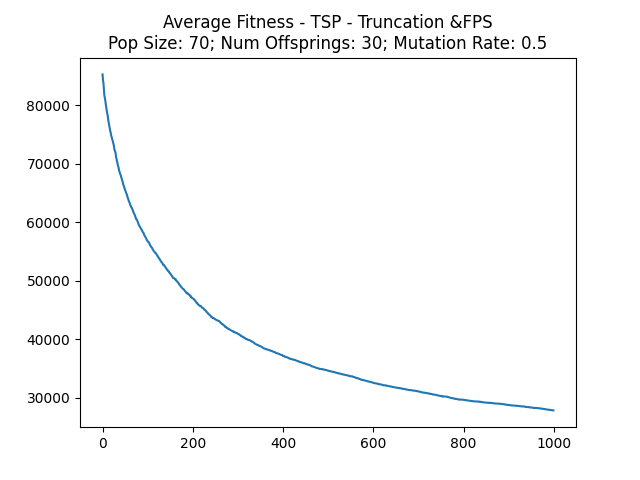
\includegraphics[width=\linewidth]{../Analysis/ASF_TSP_3_0_70_30.png}
	\end{minipage}
	\hspace{\fill}
	\begin{minipage}{0.4\textwidth}
		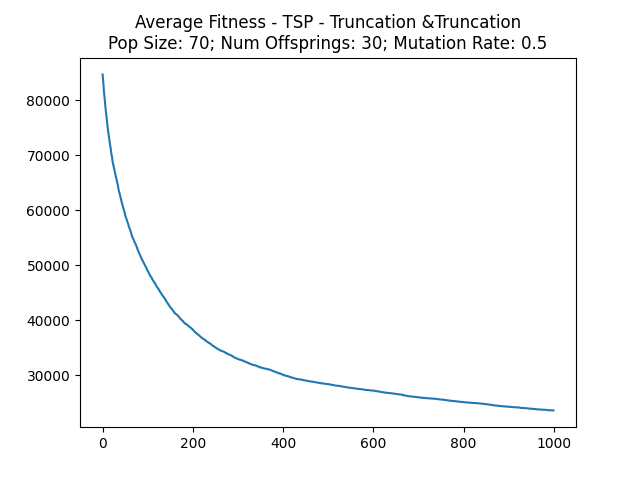
\includegraphics[width=\linewidth]{../Analysis/ASF_TSP_3_3_70_30.png}
	\end{minipage}
	\vspace*{1cm}
	\begin{minipage}{0.4\textwidth}
		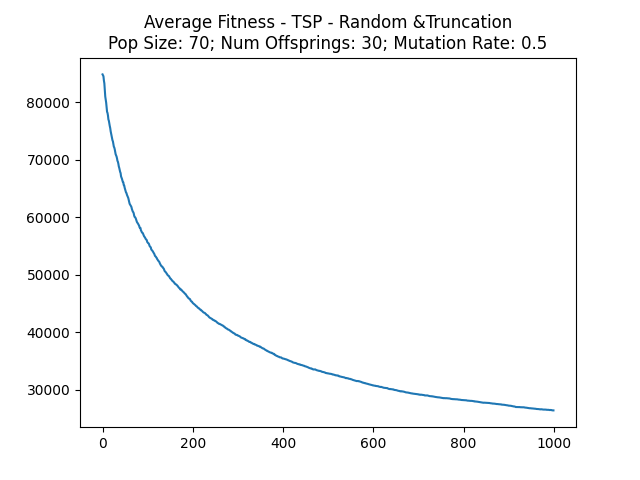
\includegraphics[width=\linewidth]{../Analysis/ASF_TSP_4_3_70_30.png}
	\end{minipage}
	\hspace{\fill}
	\begin{minipage}{0.4\textwidth}
		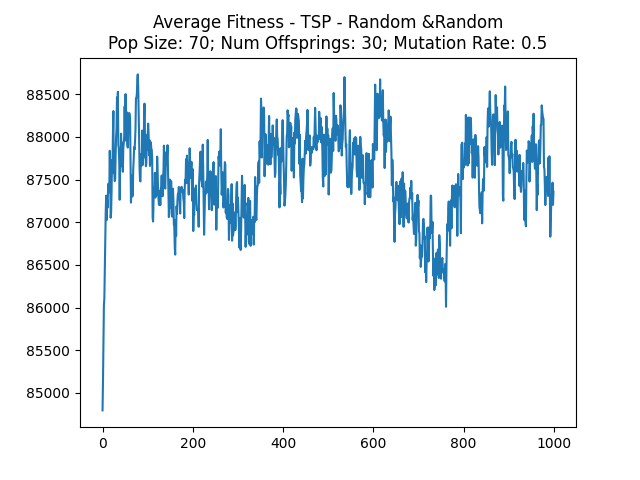
\includegraphics[width=\linewidth]{../Analysis/ASF_TSP_4_4_70_30.png}
	\end{minipage}
\end{figure}

\newpage

\subsection{Best So Far}
The best results we got from BSF were from the selection schemes FBS \& Truncation, and Tournament and RBS, where both have pretty similar and excellent results. The worst case results were from Random \& Random, FBS \& Random.

Overall if we look at the trends of the plots of our BSF plots we can see that most of our selection scheme combinations have performed.
\begin{figure}[!]
	\centering
	\begin{minipage}{0.4\textwidth}
		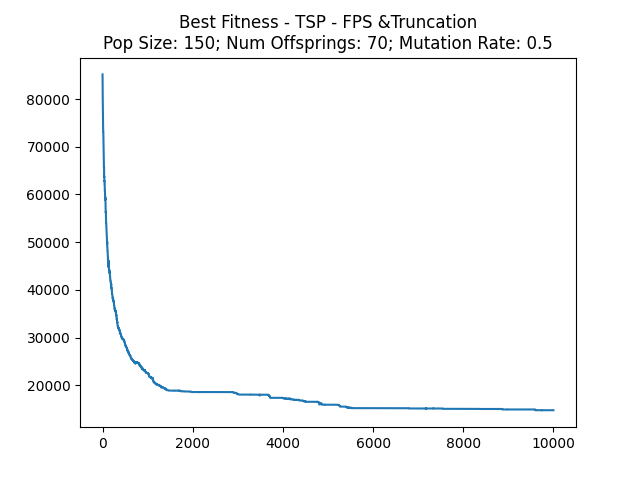
\includegraphics[width=\linewidth]{../Analysis/BSF_TSP_0_3_150_70.png}
	\end{minipage}
	\hspace{\fill}
	\begin{minipage}{0.4\textwidth}
		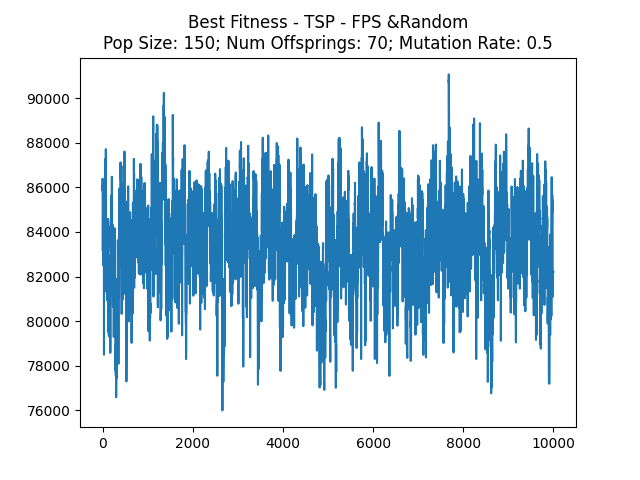
\includegraphics[width=\linewidth]{../Analysis/BSF_TSP_0_4_150_70.png}
	\end{minipage}
	\vspace*{1cm}
	\begin{minipage}{0.4\textwidth}
		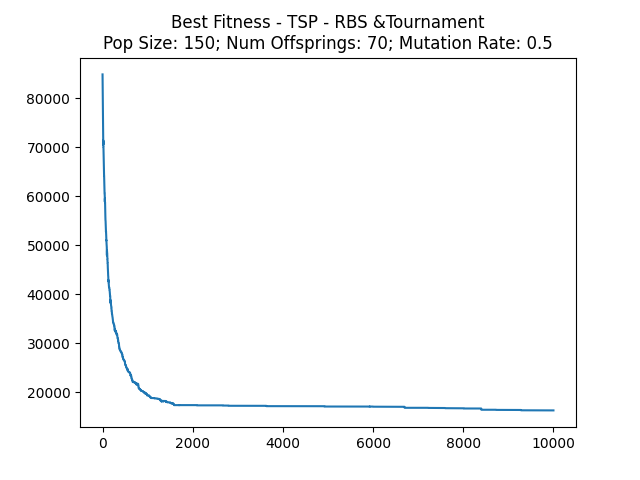
\includegraphics[width=\linewidth]{../Analysis/BSF_TSP_1_2_150_70.png}
	\end{minipage}
	\hspace{\fill}
	\begin{minipage}{0.4\textwidth}
		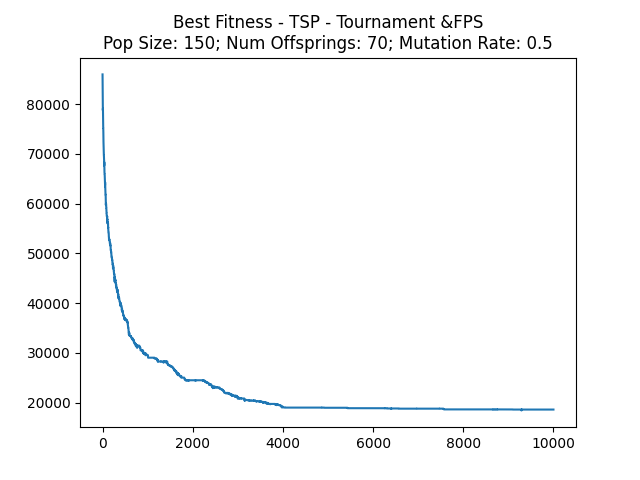
\includegraphics[width=\linewidth]{../Analysis/BSF_TSP_2_0_150_70.png}
	\end{minipage}
	\vspace*{1cm}
	\begin{minipage}{0.4\textwidth}
		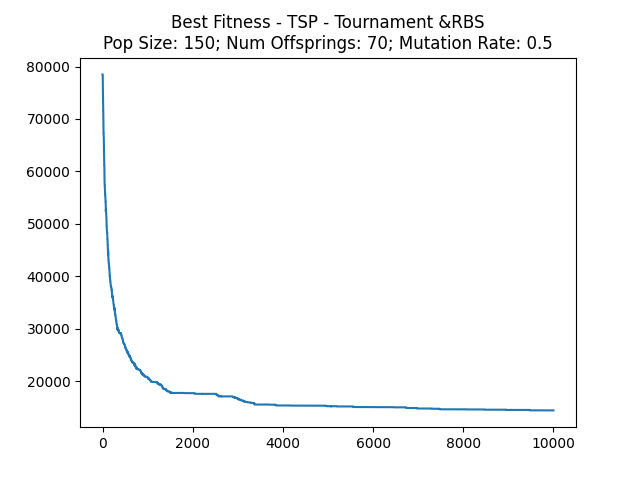
\includegraphics[width=\linewidth]{../Analysis/BSF_TSP_2_1_150_70.png}
	\end{minipage}
	\hspace{\fill}
	\begin{minipage}{0.4\textwidth}
		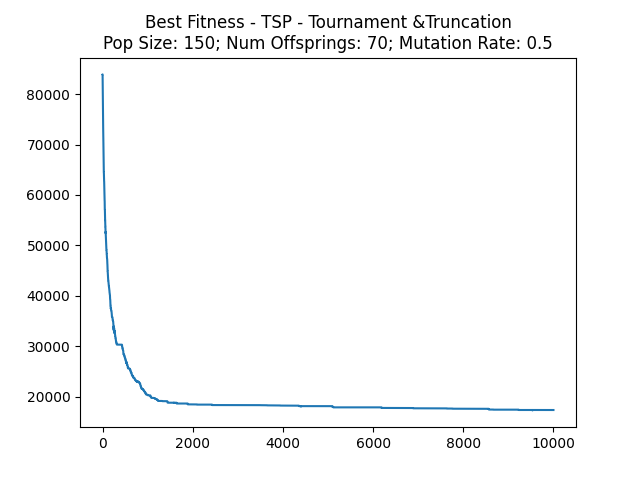
\includegraphics[width=\linewidth]{../Analysis/BSF_TSP_2_3_150_70.png}
	\end{minipage}
	\vspace*{1cm}
	\begin{minipage}{0.4\textwidth}
		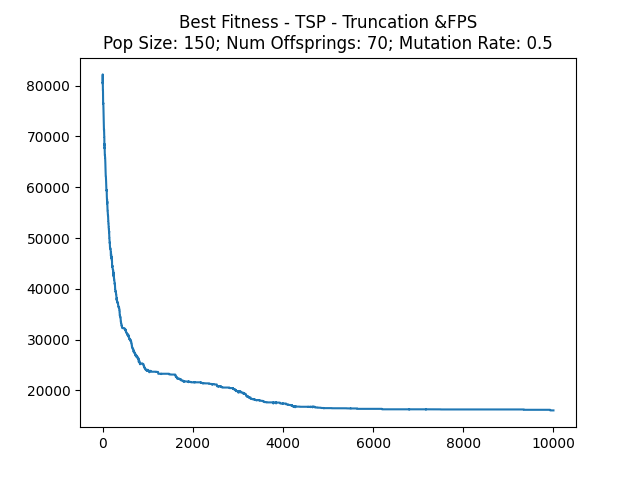
\includegraphics[width=\linewidth]{../Analysis/BSF_TSP_3_0_150_70.png}
	\end{minipage}
	\hspace{\fill}
	\begin{minipage}{0.4\textwidth}
		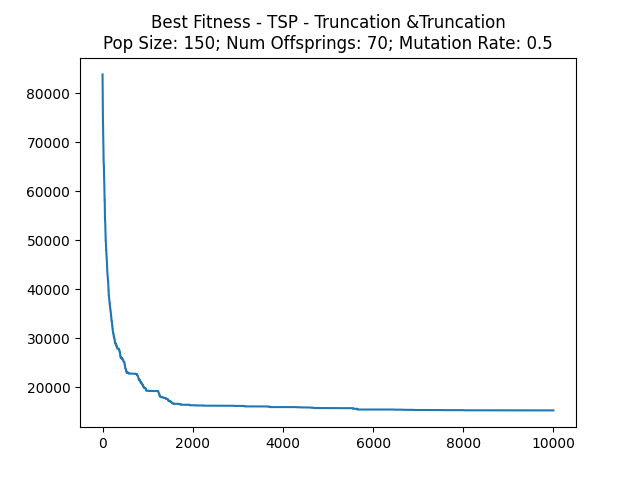
\includegraphics[width=\linewidth]{../Analysis/BSF_TSP_3_3_150_70.png}
	\end{minipage}
	\vspace*{1cm}
	\begin{minipage}{0.4\textwidth}
		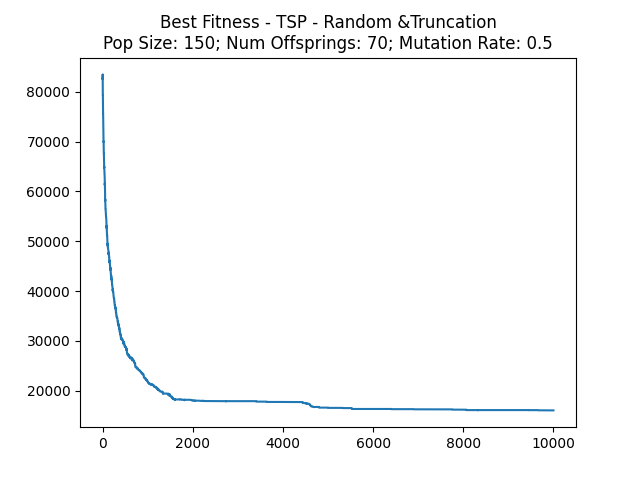
\includegraphics[width=\linewidth]{../Analysis/BSF_TSP_4_3_150_70.png}
	\end{minipage}
	\hspace{\fill}
	\begin{minipage}{0.4\textwidth}
		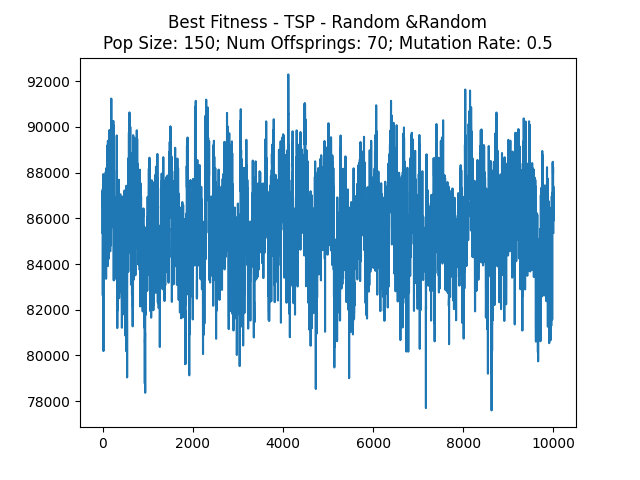
\includegraphics[width=\linewidth]{../Analysis/BSF_TSP_4_4_150_70.png}
	\end{minipage}
\end{figure}
\newpage

\section{Knapsack Problem}

\subsection{Average So Far}
Majority of the results from the selection scheme combinations were quite similar, with very few differences from each other, however, Truncation \& Truncation and Tournament \& FPS were the best, with their fitness being 9758. On the other hand, the worst selection scheme combination was of Random \& Random, moreover FPS \& Random did not have good results as compared to our other fitnesses achieved.

\begin{figure}[!]
	\begin{minipage}{0.4\textwidth}
		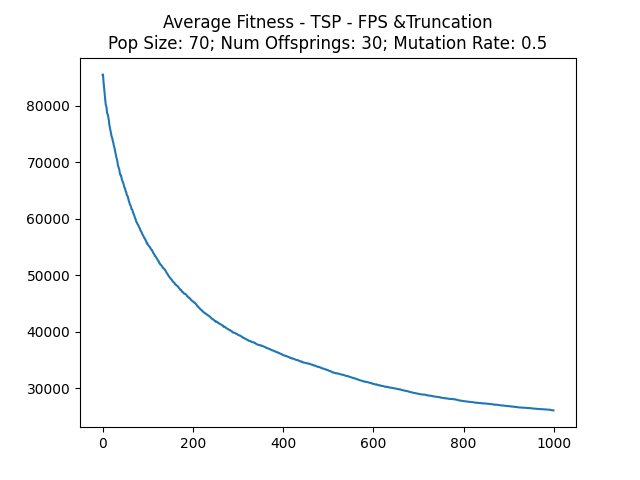
\includegraphics[width=\linewidth]{../Analysis/ASF_TSP_0_3_70_30.png}
	\end{minipage}
	\hspace{\fill}
	\begin{minipage}{0.4\textwidth}
		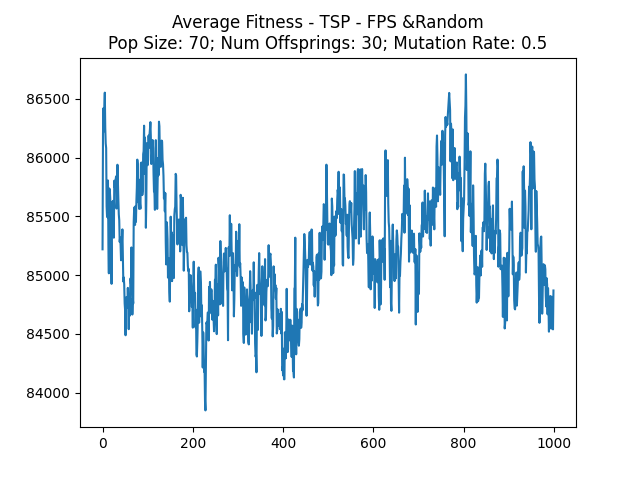
\includegraphics[width=\linewidth]{../Analysis/ASF_TSP_0_4_70_30.png}
	\end{minipage}
	\vspace*{1cm}
	\begin{minipage}{0.4\textwidth}
		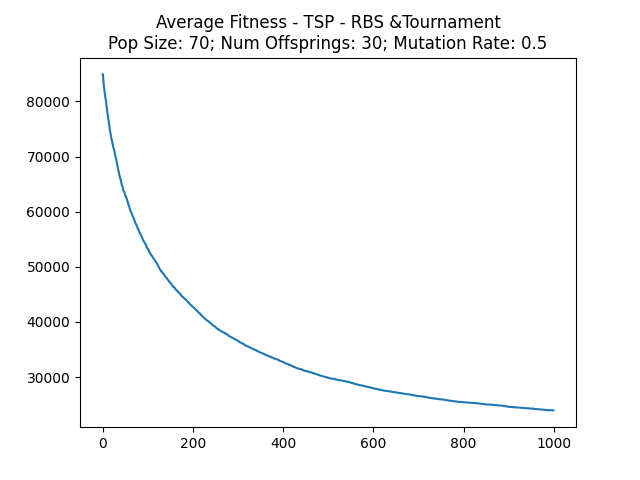
\includegraphics[width=\linewidth]{../Analysis/ASF_TSP_1_2_70_30.png}
	\end{minipage}
	\hspace{\fill}
	\begin{minipage}{0.4\textwidth}
		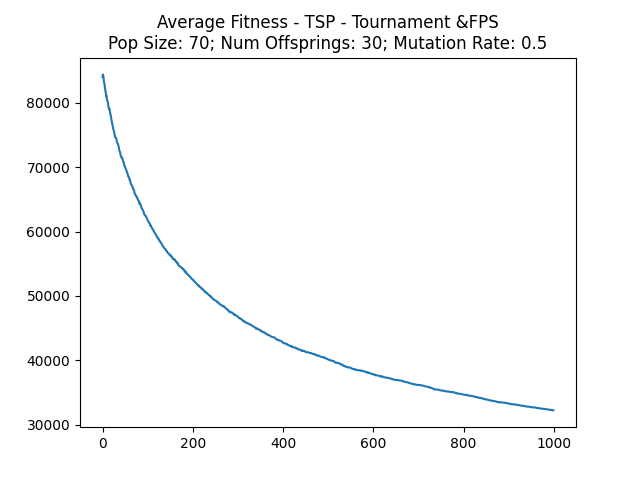
\includegraphics[width=\linewidth]{../Analysis/ASF_TSP_2_0_70_30.png}
	\end{minipage}
	\vspace*{1cm}
	\begin{minipage}{0.4\textwidth}
		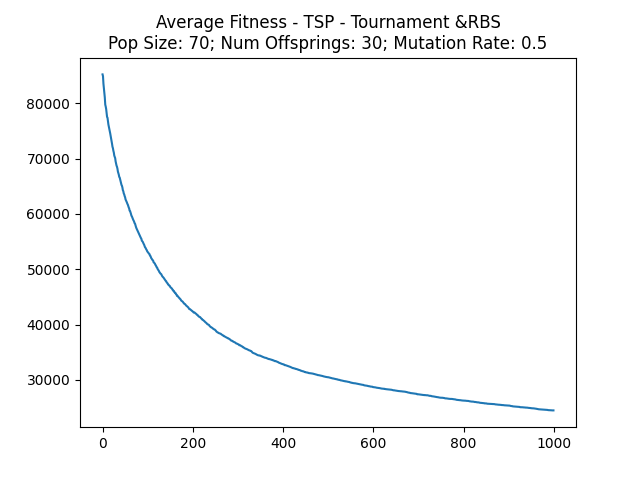
\includegraphics[width=\linewidth]{../Analysis/ASF_TSP_2_1_70_30.png}
	\end{minipage}
	\hspace{\fill}
	\begin{minipage}{0.4\textwidth}
		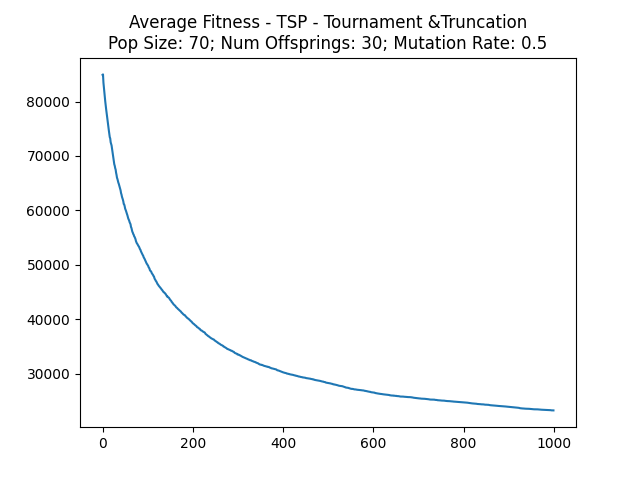
\includegraphics[width=\linewidth]{../Analysis/ASF_TSP_2_3_70_30.png}
	\end{minipage}
	\vspace*{1cm}
	\begin{minipage}{0.4\textwidth}
		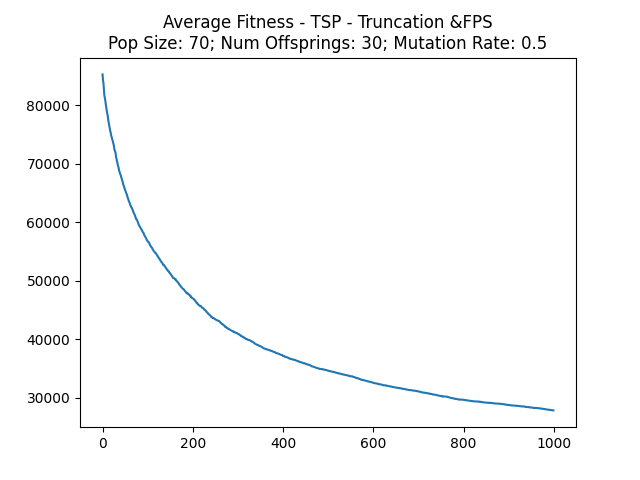
\includegraphics[width=\linewidth]{../Analysis/ASF_TSP_3_0_70_30.png}
	\end{minipage}
	\hspace{\fill}
	\begin{minipage}{0.4\textwidth}
		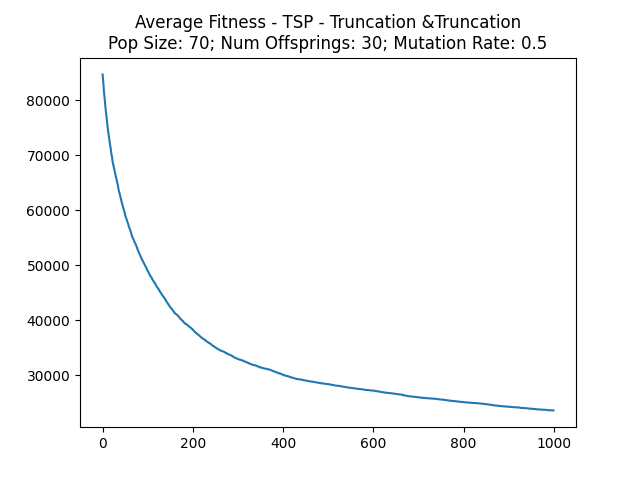
\includegraphics[width=\linewidth]{../Analysis/ASF_TSP_3_3_70_30.png}
	\end{minipage}
	\vspace*{1cm}
	\begin{minipage}{0.4\textwidth}
		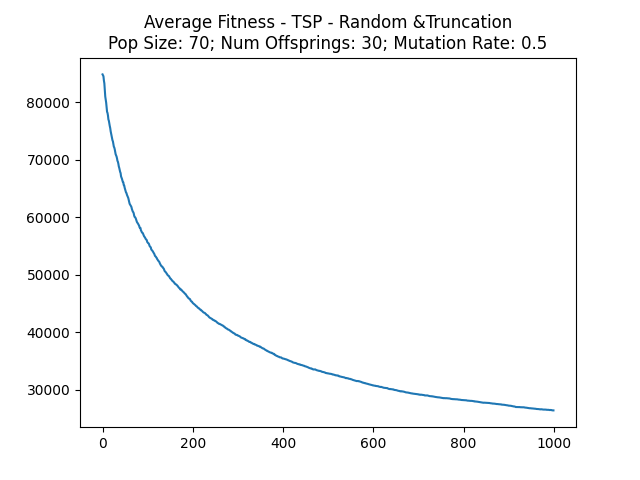
\includegraphics[width=\linewidth]{../Analysis/ASF_TSP_4_3_70_30.png}
	\end{minipage}
	\hspace{\fill}
	\begin{minipage}{0.4\textwidth}
		\includegraphics[width=\linewidth]{../Analysis/ASF_TSP_4_4_70_30.png}
	\end{minipage}
\end{figure}
\newpage

\subsection{Best So Far}
The best selection combination that we found was RBS \& Tournament, with the fitness value being 9763. The worst selection scheme combination was Random \& Random, which had no convergence , with the fitness value fluctuating between 4000-2000 throughout multiple generations


\begin{figure}[!]

	\begin{minipage}{0.4\textwidth}
		\includegraphics[width=\linewidth]{../Analysis/BSF_Knapsack_0_3_150_70.png}
	\end{minipage}
	\hspace{\fill}
	\begin{minipage}{0.4\textwidth}
		\includegraphics[width=\linewidth]{../Analysis/BSF_Knapsack_0_4_150_70.png}
	\end{minipage}
	\vspace*{1cm}
	\begin{minipage}{0.4\textwidth}
		\includegraphics[width=\linewidth]{../Analysis/BSF_Knapsack_1_2_150_70.png}
	\end{minipage}
	\hspace{\fill}
	\begin{minipage}{0.4\textwidth}
		\includegraphics[width=\linewidth]{../Analysis/BSF_Knapsack_2_0_150_70.png}
	\end{minipage}
	\vspace*{1cm}
	\begin{minipage}{0.4\textwidth}
		\includegraphics[width=\linewidth]{../Analysis/BSF_Knapsack_2_1_150_70.png}
	\end{minipage}
	\hspace{\fill}
	\begin{minipage}{0.4\textwidth}
		\includegraphics[width=\linewidth]{../Analysis/BSF_Knapsack_2_3_150_70.png}
	\end{minipage}
	\vspace*{1cm}
	\begin{minipage}{0.4\textwidth}
		\includegraphics[width=\linewidth]{../Analysis/BSF_Knapsack_3_0_150_70.png}
	\end{minipage}
	\hspace{\fill}
	\begin{minipage}{0.4\textwidth}
		\includegraphics[width=\linewidth]{../Analysis/BSF_Knapsack_3_3_150_70.png}
	\end{minipage}
	\vspace*{1cm}
	\begin{minipage}{0.4\textwidth}
		\includegraphics[width=\linewidth]{../Analysis/BSF_Knapsack_4_3_150_70.png}
	\end{minipage}
	\hspace{\fill}
	\begin{minipage}{0.4\textwidth}
		\includegraphics[width=\linewidth]{../Analysis/BSF_Knapsack_4_4_150_70.png}
	\end{minipage}
\end{figure}


\end{document}